\section{Martin Andleberger}

\begin{center}
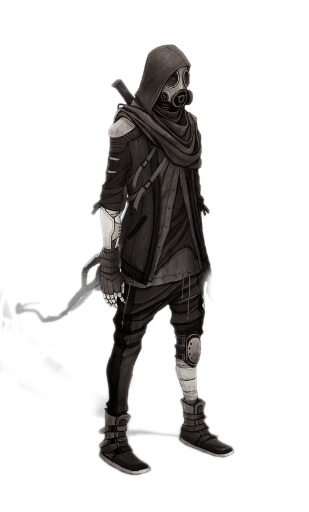
\includegraphics[width=80mm]{./content/img/martin.png}
\begin{figure}[h]
\end{figure}
\end{center}

\subsection*{Details}

\noindent

Race: 	Construct (Craftwerk) \\
Class: 	Bard/Sorcerer \\
Age: 	87 \\
Status: Active (sometimes a mouse)

\subsubsection{Background}

The Andelbergers seemed like any other old aristocratic family from Linderdorf, at least from the outside.  Who was to know that the family line stretched almost a thousand years back in history, so far back that the family's origins predated the Sundering itself.

Lord and Lady Andelberger had been maintaining a pure bloodline ever since the Sundering, and the latest generation had proved very difficult indeed, the Lady had only managed to produce a single child, a solitary young woman who glowed with the radiance of Hemotate.  She was schooled from the family's great library, and a sense of destiny passed into her.  Until one dark and stormy night the Church arrived, or at least the part of the Church that people only talked about in whispers.  Dark masked figures stormed the house and decimated what was left of the family.  What happened to the young Ms Andelberger remains unknown.

Martin was the family's fighting butler, built using the knowledge of the ancient family line to protect and serve Ms Andelberger and keep her entertained.  His clothes and parts were shaped in strange swirling patterns taken from books long considered useless.  On the fateful night the Inquisition appeared, Martin was out milking the cows in the freezing rain.  He missed the entire saga, returning only to an empty house torn apart at the seams.  He rescued his favourite books and weighed up his options.  He had lost everything, but he still had two purposes: to find the young Ms Andelberger, and to avenge the family line.  As possibly the last member of the Andelberger household, it fell to him to return the gods to their rightful place within the pantheon.

All this was almost a century ago.  Unable to die, the butler wandered the streets, then the town, then the city, and finally the continent, until he was found beaten and chained up by Varg bearkin in the frozen north, and chanced upon by a motley crew in an airship.

\subsubsection{Personality and Traits}

Martin was deeply depressed when the party found him, lacking the spark of power that had once helped him deal with the day-to-day drudgery of being immortal.  When he discovered the group's goal was to destroy the Church, he picked himself up only a little bit.  It was not until he learned that his ward Ms Andelberger had ascended to the heavens that he doubled down and vowed vengeance.

His face and most of his skin were partly metal, fashioned with craftwerk precision.  He had a cable-hand that could extend for grappling, used most dramatically to rescue Kevin from the frozen Varg wastes, and could transform into a small mouse form, which he used with alarming regularity.  Before the arena fight against the Stonecast Mech, Mr Mouse climbed out to rub dirt in two lines under his eyes before climbing back in.  Hardcore.

Martin stuttered badly when he was first found, a defect that Burnie fixed with a quick shock from his electrical gloves.  He spoke Tikki Tuck, Goblin, and Low Velterran, and had been quietly teaching Myron vocabulary in his sleep, steadily improving the gnome's eloquence without his knowledge.

He claimed to have an imaginary girlfriend in Nanduan.  Kevin insisted his own girlfriend was real.

\subsubsection{Relationships}

Martin became most attached to Burnie of all the party members, the gruff old Book Burner's practical nature apparently appealing to the construct's sensibilities.  Burnie was the one who fixed his stutter, recharged him in the field, and treated him as a capable ally rather than a curiosity.

His relationship with the wider group was complicated by suspicion.  Myron harboured serious doubts about whether Martin was truly on their side or on some other mission, and the two had tense exchanges, though their silent hour-long walk together before the Festival of Light suggested a mutual understanding beneath the friction.  When Martin tried to kill the rescued Arbiter Kiros inside Seven's Spire, believing all Church members deserved death, it was Myron who pinned him to the ground.  Exmerah took him aside afterwards and explained that, barring herself, every member of the party had worked for the Church at some point, a revelation that left him flabbergasted.

Martin made a deal with Lazarus in Hell, agreeing to do whatever the devil wanted in exchange for help finding answers about his lost ward.  The exact terms were characteristically vague.

\subsubsection{Martin's Story}

Martin was found chained up and being beaten by Varg bearkin in the frozen north, barely conscious and kept upright only by the chains attached to nearby trees.  Kevin and the party rescued him, though Martin initially refused to join them, attempting to jump off the airship on multiple occasions.  When the gnome inventors aboard recognised him as an official member of a northern expedition, his cover was blown and he reluctantly stayed.

He proved his worth in the climb to the Bright Bart Forge, charging himself from a lightning strike and unleashing torrents of electricity at the Aspect of the Storm, an air elemental wielding a lightning sword that had sealed the forge for centuries.  Though the overload tore him to pieces, Burnie recharged him just in time.  At the forge, Martin helped the party claim the ancient forging tools, rune-carving books, and materials that would be used to create their Excalibrum weapons.

In Linderdorf, Martin put his craftwerk expertise to use, building new weapons and exoskeletons for the party and scouting the Stonecast Mech in the Clawtech arena, convincing its owners to disassemble and reassemble it before the fight, quietly sabotaging its readiness.  During the arena battle itself, Martin threw storm spheres from inside the Mech's cockpit-sized mouse compartment, his lightning striking aggressively against the arena walls to wild cheering.  After Myron's bisecting final blow, it was Martin who supplied the word the gnome was reaching for, and who threw glitter into the air as he thunderstepped out while three-quarters of the crowd chanted ``EMANCIPATION!''

Martin's calculations for the assault on Seven's Spire proved correct, the airship could indeed destroy the tower, though the ship might not survive the impact.  He disguised himself as Lazarus for the Festival of Light infiltration, and inside the Spire he made STANRI invisible by disconnecting and reconnecting its mechanical systems and infusing it with fey wild magic, creating the ``invisible bear'' that blocked enemy escape routes while the party fought through floor after floor toward the pinnacle.

\begin{DndSidebar}{Mr Mouse}
Martin's mouse form became the group's secret weapon.  He scouted enemy positions from inside walls, climbed into the Stonecast Mech's head compartment to pilot it, and received cheese from Exme as payment for services rendered.  The transformation process, a construct butler folding himself down into a small rodent, was never adequately explained and nobody thought to ask.
\end{DndSidebar}

\clearpage